%%%%%%%%%%%%%%%%%%%%%%%%%%%%%%%%%%%%%%%%%%%%%%%%%%%%%%%%
% 							                   PREAMBULE        
%%%%%%%%%%%%%%%%%%%%%%%%%%%%%%%%%%%%%%%%%%%%%%%%%%%%%%%%

\documentclass[a4,12pt]{article}

%--- Packages génériques ---%

\usepackage[francais]{babel}
\usepackage[utf8]{inputenc}
\usepackage[T1]{fontenc}
\usepackage[babel=true]{csquotes}
\usepackage{amsmath}
\usepackage{amssymb}
\usepackage{float}
\usepackage{graphicx}
\usepackage{hyperref}

%--- Structure de la page ---%

\usepackage{fancyheadings}

\topmargin -1.5 cm
\oddsidemargin -0.5 cm
\evensidemargin -0.5 cm
\textwidth 17 cm
\setlength{\headwidth}{\textwidth}
\textheight 24 cm
\pagestyle{fancy}
\lhead[\fancyplain{}{\thepage}]{\fancyplain{}{\sl ENSIMAG 2A}}
\chead[\fancyplain{}{{\sl }}]{\fancyplain{}{{TP Traitement d'Image}}}
\rhead[\fancyplain{}{}]{\fancyplain{}{Loiodice \& Vincent}}
\lfoot{\fancyplain{}{}}
\cfoot{\fancyplain{}{}}
\cfoot{\thepage }
\rfoot{\fancyplain{}{}}

%--- Style de la zone de code ---%

\usepackage{tikz}
\usetikzlibrary{calc}
\usepackage[framemethod=tikz]{mdframed}
\usepackage{listings}             
\usepackage{textcomp}

\lstset{upquote=true,
        columns=flexible,
        keepspaces=true,
        breaklines,
        breakindent=0pt,
        basicstyle=\ttfamily,
        commentstyle=\color[rgb]{0,0.6,0},
        language=Scilab,
        alsoletter=\),
        }

\lstset{classoffset=0,
        keywordstyle=\color{violet!75},
        deletekeywords={zeros,disp},
        classoffset=1,
        keywordstyle=\color{cyan},
        morekeywords={zeros,disp},
        }

\lstset{extendedchars=true,
        literate={0}{{\color{brown!75}0}}1 
                 {1}{{\color{brown!75}1}}1 
                 {2}{{\color{brown!75}2}}1 
                 {3}{{\color{brown!75}3}}1 
                 {4}{{\color{brown!75}4}}1 
                 {5}{{\color{brown!75}5}}1 
                 {6}{{\color{brown!75}6}}1 
                 {7}{{\color{brown!75}7}}1 
                 {8}{{\color{brown!75}8}}1 
                 {9}{{\color{brown!75}9}}1 
                 {(}{{\color{blue!50}(}}1 
                 {)}{{\color{blue!50})}}1 
                 {[}{{\color{blue!50}[}}1 
                 {]}{{\color{blue!50}]}}1
                 {-}{{\color{gray}-}}1
                 {+}{{\color{gray}+}}1
                 {=}{{\color{gray}=}}1
                 {:}{{\color{orange!50!yellow}:}}1
                 {é}{{\'e}}1 
                 {è}{{\`e}}1 
                 {à}{{\`a}}1 
                 {ç}{{\c{c}}}1 
                 {œ}{{\oe}}1 
                 {ù}{{\`u}}1
                 {É}{{\'E}}1 
                 {È}{{\`E}}1 
                 {À}{{\`A}}1 
                 {Ç}{{\c{C}}}1 
                 {Œ}{{\OE}}1 
                 {Ê}{{\^E}}1
                 {ê}{{\^e}}1 
                 {î}{{\^i}}1 
                 {ô}{{\^o}}1 
                 {û}{{\^u}}1 
        }

%--- Raccourcis commande ---%

\newcommand{\R}{\mathbb{R}}
\newcommand{\N}{\mathbb{N}}
\newcommand{\A}{\mathbf{A}}
\newcommand{\B}{\mathbf{B}}
\newcommand{\C}{\mathbf{C}}
\newcommand{\D}{\mathbf{D}}
\newcommand{\ub}{\mathbf{u}}

%--- Mode correction et incréments automatiques ---%

\usepackage{framed}
\usepackage{ifthen}
\usepackage{comment}
\usepackage{graphicx}

\newcounter{Nbquestion}

\newcommand*\question{%
\stepcounter{Nbquestion}%
\textbf{Question \theNbquestion. }}

\newboolean{enseignant}
%\setboolean{enseignant}{true}
\setboolean{enseignant}{false}

\definecolor{shadecolor}{gray}{0.80}

\ifthenelse{
\boolean{enseignant}}{
\newenvironment{correction}{\begin{shaded}}{\end{shaded}}
}
{
\excludecomment{correction}
}

%--- Style de l'encadré des questions ---%

\mdfsetup{leftmargin=12pt}
\mdfsetup{skipabove=\topskip,skipbelow=\topskip}

\tikzset{
	warningsymbol/.style={
	rectangle,draw=red,
	fill=white,scale=1,
	overlay}}
\global\mdfdefinestyle{exampledefault}{
	hidealllines=true,leftline=true,
	innerrightmargin=0.0em,
	innerleftmargin=0.3em,
	leftmargin=0.0em,
	linecolor=red,
	backgroundcolor=orange!20,
	middlelinewidth=4pt,
	innertopmargin=\topskip,
}

\global\mdfdefinestyle{answer}{
	hidealllines=true,leftline=true,
	innerrightmargin=0.0em,
	innerleftmargin=0.3em,
	leftmargin=0.0em,
	linecolor=green,
	backgroundcolor=white,
	middlelinewidth=4pt,
	innertopmargin=\topskip,
}

%%%%%%%%%%%%%%%%%%%%%%%%%%%%%%%%%%%%%%%%%%%%%%%%%%%%%%%%
% 							               EN-TETE        
%%%%%%%%%%%%%%%%%%%%%%%%%%%%%%%%%%%%%%%%%%%%%%%%%%%%%%%%

\title{\textbf{TP1 Traitement d'Image\\Convolution : Lissage et détection de contours}}
\author{
\begin{tabular}{cc}
	\textsc{Loiodice Thomas} & \textsc{Vincent Kylian} \\
\end{tabular}}   
\date{\small \today}

\makeatletter
	\def\thetitle{\@title}
	\def\theauthor{\@author}
	\def\thedate{\@date}
\makeatother 

\usepackage{etoolbox}
\usepackage{titling}
\setlength{\droptitle}{-7em}

\setlength{\parindent}{1cm}

\makeatletter
% patch pour le bug concernant les parenthèses fermantes d'après http://tex.stackexchange.com/q/69472
\patchcmd{\lsthk@SelectCharTable}{%
  \lst@ifbreaklines\lst@Def{`)}{\lst@breakProcessOther)}\fi}{}{}{}
  
%%%%%%%%%%%%%%%%%%%%%%%%%%%%%%%%%%%%%%%%%%%%%%%%%%%%%%%%
% 							CORPS DU DOCUMENT          
%%%%%%%%%%%%%%%%%%%%%%%%%%%%%%%%%%%%%%%%%%%%%%%%%%%%%%%%

\begin{document}
\maketitle


%%%%%%%%%%%%%%%%%%%%%%%%%%%%%%%%%%%%%%%%%%%%%%%%%%%%%%%%
% 						                  	PARTIE I         
%%%%%%%%%%%%%%%%%%%%%%%%%%%%%%%%%%%%%%%%%%%%%%%%%%%%%%%%

\section{Partie I : Lissage linéaire}

\subsection{FFT et filtrage fréquentiel}


En étudiant les résultats obtenus sur les différents types de bruit nous avons vu que ce filtrage est plus adapté à certains types de bruit que d'autres. En effet le filtre semble être efficace sur les bruits gaussien et speckle mais semble moins adapté au bruit poivre et sel.\\

L'estimation d'un résultat visuel est parfois compliqué, en effet le "meilleur" lissage est difficile à choisir : plus le lissage est fort plus les couleurs sont constantes et proches des images d'origine mais plus les contours deviennent épais et flous. Ainsi dans nos estimations visuelles nous avions souvent choisi un $\sigma$ plus faible que celui maximisant le PSNR.\\


Exemple pour l'image \textit{figure2bb50.pgm} :\\

\noindent
\begin{minipage}[c]{0.20\linewidth}
	\begin{center}
		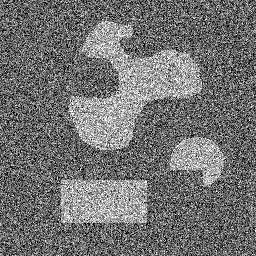
\includegraphics[width = 33mm]{./img/formes2bb50.jpg}
		\textit{origine}
	\end{center}
\end{minipage}
\begin{minipage}[c]{0.20\linewidth}
	\begin{center}
		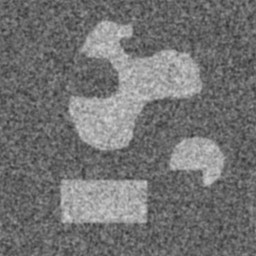
\includegraphics[width = 33mm]{./img/2bb50-1.jpg}
		\textit{$\sigma = 1$}
	\end{center}
\end{minipage}
\begin{minipage}[c]{0.20\linewidth}
	\begin{center}
		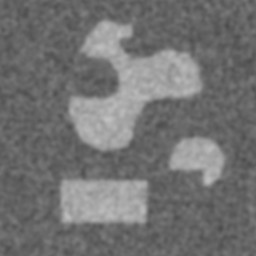
\includegraphics[width = 33mm]{./img/2bb50-2.jpg}
		\textit{$\sigma = 2$}
	\end{center}
\end{minipage}
\begin{minipage}[c]{0.20\linewidth}
	\begin{center}
		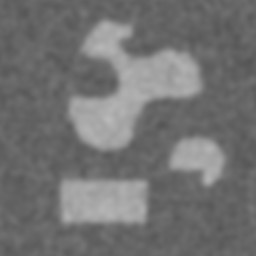
\includegraphics[width = 33mm]{./img/2bb50-3.jpg}
		\textit{$\sigma = 3$}
	\end{center}
\end{minipage}
\begin{minipage}[c]{0.20\linewidth}
	\begin{center}
		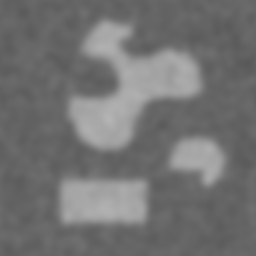
\includegraphics[width = 33mm]{./img/2bb50-4.jpg}
		\textit{$\sigma = 4$}
	\end{center}
\end{minipage}


\subsubsection*{Bruit gaussien}
Ce bruit, caractérisé par un flou et l'addition d'un bruit blanc, nous a semblé être le plus réceptif au lissage. Avec l'image \textit{formes2bb40.pgm} on obtient les résultats suivants :
\begin{center}
\begin{minipage}[c]{0.30\linewidth}
	\begin{center}
		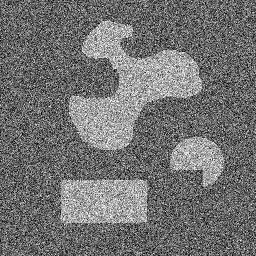
\includegraphics[width = 50mm]{./img/2bb40.jpg}
		\textit{origine}\\
		\textit{PSNR = 16.36}
	\end{center}
\end{minipage}
\begin{minipage}[c]{0.30\linewidth}
	\begin{center}
		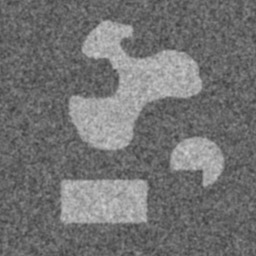
\includegraphics[width = 50mm]{./img/2bb40-1.jpg}
		\textit{$\sigma = 1$}\\
		\textit{PSNR = 26.86}
	\end{center}
\end{minipage}
\begin{minipage}[c]{0.30\linewidth}
	\begin{center}
		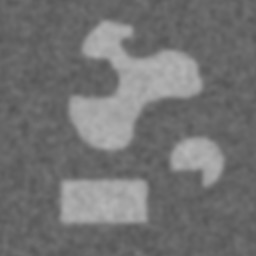
\includegraphics[width = 50mm]{./img/2bb40-2_5.jpg}
		\textit{$\sigma = 2.5$}\\
		\textit{PSNR = 30.29}
	\end{center}
\end{minipage}
\end{center}

Le résultat obtenu permet d'obtenir un bon PSNR dès $\sigma=1$, cette valeur nous a semblé un bon compromis entre le lissage et l'apparition de flou, cependant le PSNR maximal peut être obtenu pour $\sigma=2.5$.


\subsubsection*{Bruit speckle}
Le bruit speckle semble
Nous avons pris une image qui nous a semblé proche qualitativement et quantitativement niveau bruit de l'image testée en section précédente (\textit{formes2bb40.pgm}) pour le buit speckle : l'image \textit{formes2sp1.pgm}.
\begin{center}
	\begin{minipage}[c]{0.30\linewidth}
		\begin{center}
			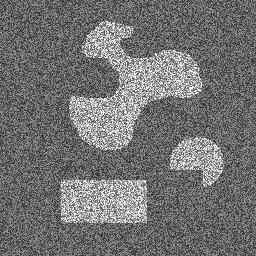
\includegraphics[width = 50mm]{./img/2sp1.jpg}
			\textit{origine}\\
			\textit{PSNR = 16.77}
		\end{center}
	\end{minipage}
	\begin{minipage}[c]{0.30\linewidth}
		\begin{center}
			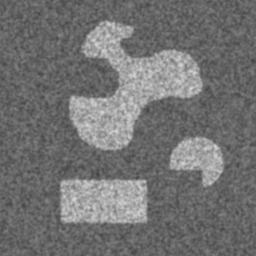
\includegraphics[width = 50mm]{./img/2sp1-1.jpg}
			\textit{$\sigma = 1$}\\
			\textit{PSNR = 27.23}
		\end{center}
	\end{minipage}
	\begin{minipage}[c]{0.30\linewidth}
		\begin{center}
			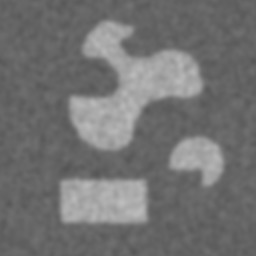
\includegraphics[width = 50mm]{./img/2sp1-2_4.jpg}
			\textit{$\sigma = 2.4$}\\
			\textit{PSNR = 30.52}
		\end{center}
	\end{minipage}\\
\end{center}

Ici le meilleur résultat est obtenu pour $\sigma=2.4$ et les résultats obtenus sont très proches de ceux pour un bruit gaussien.


\subsubsection*{Bruit poivre et sel}
Le bruit poivre et sel est celui qui résiste le plus à notre filtrage. Étant constitué de points de forte disparité (blancs et noirs, aux extrêmes de l'échelle de couleur) face aux pixels de l'image, ceux-ci ne sont lissés dans l'image qu'au prix d'un fort flou sur les contours. Pour illustrer cela nous avons choisi l'image \textit{formes1pets5.pgm}.
\begin{center}
	\begin{minipage}[c]{0.30\linewidth}
		\begin{center}
			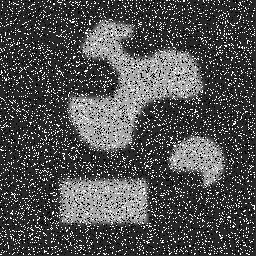
\includegraphics[width = 50mm]{./img/1pets5.jpg}
			\textit{origine}\\
			\textit{PSNR = 11.06}
		\end{center}
	\end{minipage}
	\begin{minipage}[c]{0.30\linewidth}
		\begin{center}
			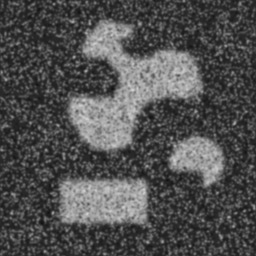
\includegraphics[width = 50mm]{./img/1pets5-1.jpg}
			\textit{$\sigma = 1$}\\
			\textit{PSNR = 18.94}
		\end{center}
	\end{minipage}
	\begin{minipage}[c]{0.30\linewidth}
		\begin{center}
			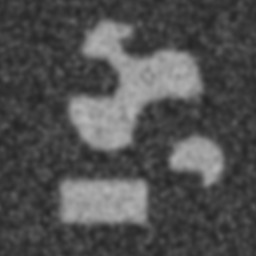
\includegraphics[width = 50mm]{./img/1pets5-2_4.jpg}
			\textit{$\sigma = 2.4$}\\
			\textit{PSNR = 20.49}
		\end{center}
	\end{minipage}
\end{center}

L'image est ici, d'origine, bien plus bruitée que les images utilisées précédemment dans les tests mais cela montre la persistance des points de bruits poivre et sel face au filtrage.

\subsection{Convolution spatiale}

Nous avons tout d'abord observé que plus le sigma est choisi grand, plus la taille de la fenêtre doit être importante pour observer les mêmes résultats qu'avec un filtrage fréquentiel. En effet, plus la valeur du lissage $\sigma$ est grande, plus la gaussienne va être étalée et sa décroissance lente. Ainsi afin de prendre en compte tous les coefficients non nuls du filtre gaussien, il sera nécessaire de prendre en compte des pixels plus éloignés du pixel calculé, et donc d'élargir la fenêtre W.\\

Cet effet est notamment visible sur le traitement ci-dessous de l'image \textit{formes1pets5.pgm} avec $\sigma = 5$ :\\

\noindent
\begin{minipage}[c]{0.50\linewidth}
	\begin{center}
		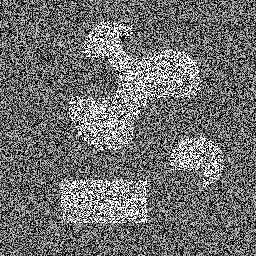
\includegraphics[width = 65mm]{./img/2sp5.jpg}\\
		\textit{Image bruitée}\\
		\textit{$PSNR_{formes1}=10.58$}
	\end{center}
\end{minipage}
\begin{minipage}[c]{0.50\linewidth}
	\begin{center}
		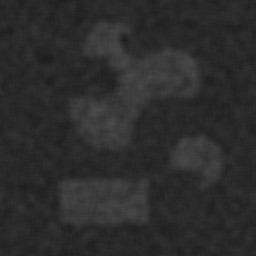
\includegraphics[width = 65mm]{./img/2sp5-5-5}\\
		\textit{$\sigma=5$ et W=5}\\
		\textit{$PSNR_{formes1}=10.93$}
	\end{center}
\end{minipage}\\
\\
Sur la figure de droite où l'on a choisi une fenêtre de taille 5, l'image est clairement assombrie, les contributions des pixels éloignés mais n'étant pas annulés par la gaussienne ne sont en effet pas prises en compte. En choisissant une fenêtre plus importante ($W = 20$), on obtient un résultat équivalent au résultat obtenu par FFT :\\

\noindent
\begin{minipage}[c]{0.50\linewidth}
	\begin{center}
		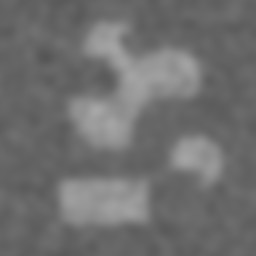
\includegraphics[width = 65mm]{./img/2sp5-5-20.jpg}\\
		\textit{$\sigma=5$ et W=20}\\
		\textit{$PSNR_{formes1}=25.91$}
	\end{center}
\end{minipage}
\begin{minipage}[c]{0.50\linewidth}
	\begin{center}
		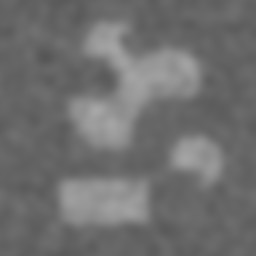
\includegraphics[width = 65mm]{./img/2sp5-5.jpg}\\
		\textit{Avec FFT, $\sigma=5$}\\
		\textit{$PSNR_{formes1}=25.91$}
	\end{center}
\end{minipage}\\
\\

Ainsi, nous avons étudié sur des exemples l'écart absolu entre le résultat obtenu par un filtrage fréquentiel et celui obtenu par un filtrage spatial en fonction de la taille de fenêtre utilisée. Nous avons choisi pour celà les images bruitées \textit{formes1pest5.pgm}, \textit{formes2sp5.pgm} \textit{formes2bb67.pgm} afin d'expérimenter les variations sur des images de contrastes et bruits différents.

Nous avons choisi des images présentant un niveau de bruit assez élevé pour permettre une bonne visualisation du filtrage.

\begin{center}
	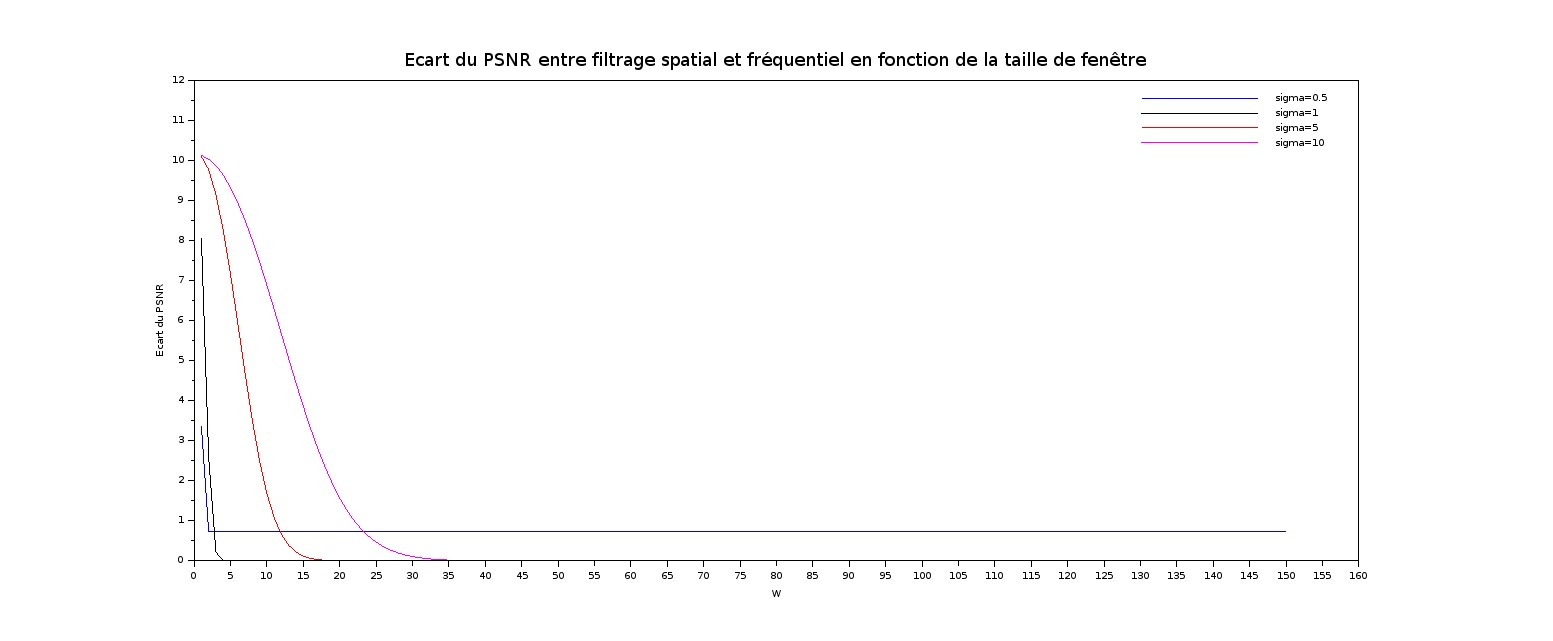
\includegraphics[width = 170mm]{./img/1pets5sce.jpg}\\
	\textit{Comparaison sur l'image formes1pets5.pgm}
\end{center}
\vspace{1cm}

\begin{center}
	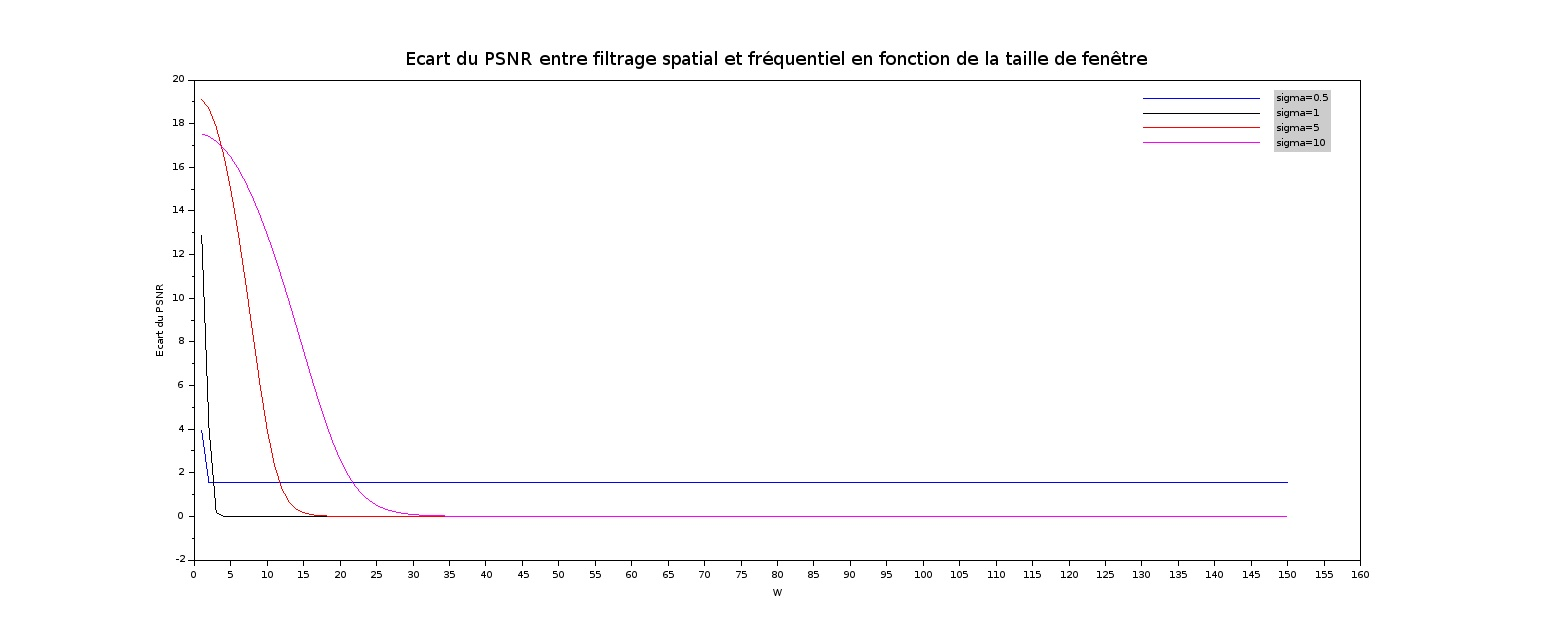
\includegraphics[width = 170mm]{./img/2sp5sce.jpg}\\
	\textit{Comparaison sur l'image formes2sp5.pgm}
\end{center}
\vspace{1cm}

\begin{center}
	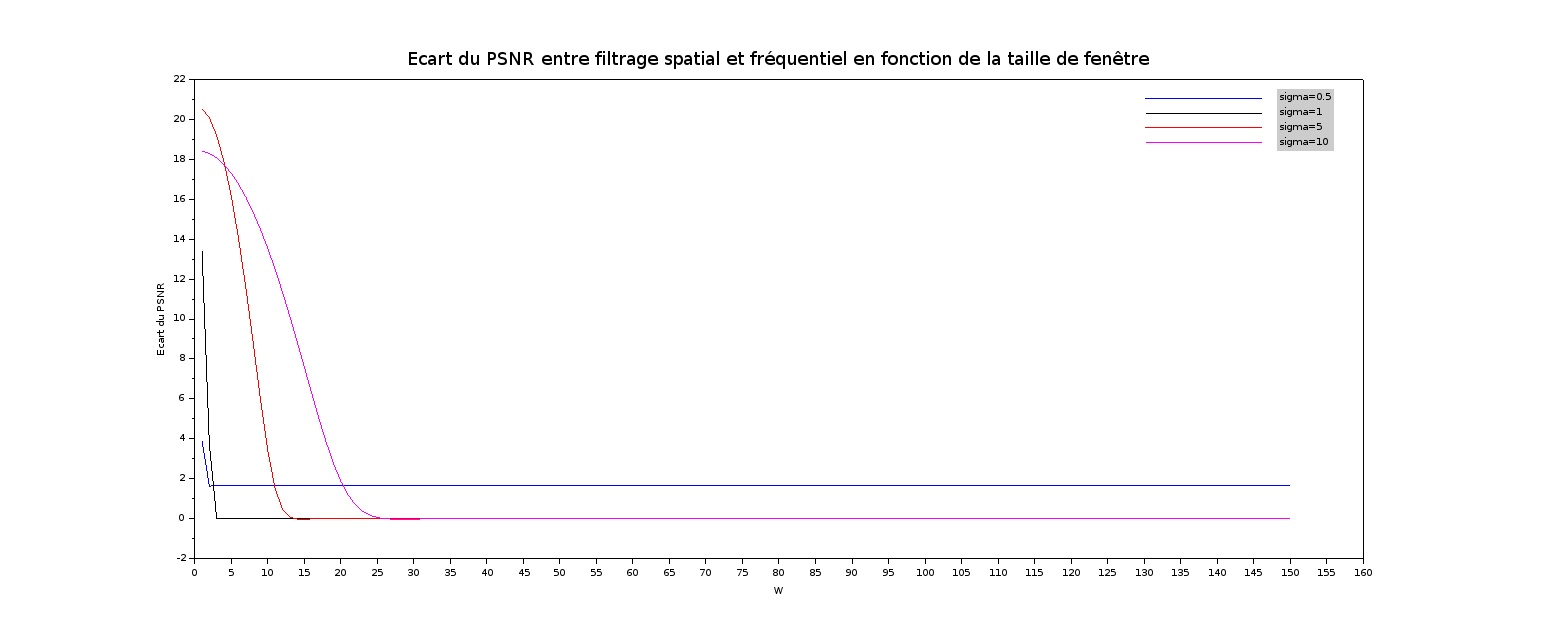
\includegraphics[width = 170mm]{./img/2bb67sce.jpg}\\
	\textit{Comparaison sur l'image formes2bb67.pgm}
\end{center}

\noindent
Ainsi on peut voir que :
\begin{itemize}
	\item Il n'est pas nécessaire d'avoir un masque d'une largeur très importante, en effet dès une taille de 40 pour les quatre valeurs de $\sigma$ testées, le résultat est identique à celui obtenu par FFT.
	\item On peut déduire de ces expérimentations une loi empirique reliant $\sigma$ et $W$ :\\
	\begin{center}
		\fbox{$W(\sigma) \geq 3 \sigma$}
	\end{center}
\end{itemize}

\vspace{1em}
On peut remarquer que pour $\sigma=0.5$, et plus généralement $\sigma < 1$, on obtient un écart qui ne tend pas vers $0$ et reste à une valeur fixe, ceci est le même phénomène pour toutes les images. Nous ne parvenons pas à expliquer cet écart non présent pour les autres valeurs.

\subsection{Complexité et comparaison des 2 méthodes}
Pour la comparaison du temps de calcul nous avons utilisé l'image \textit{formes2bb50.pgm} avec les résultats précédents, soit une taille de masque telle que $W=3\sigma$.

Nous avons ainsi comparé les temps relatifs entre l'implémentation fréquentielle (en prenant en compte le surcoût de passage par la FFT, le shift et les opérations inverses) et celle spatiale (implémentée par un filtre séparable). L'écart relatif a été calculé ainsi :\\

\begin{equation}
E_{f/s}=100\frac{T_{freq}-T_{spat}}{T_{freq}}
\end{equation}

\vspace {2em}
La figure obtenue, moyennée sur 5 mesures, est la suivante :
\begin{center}
	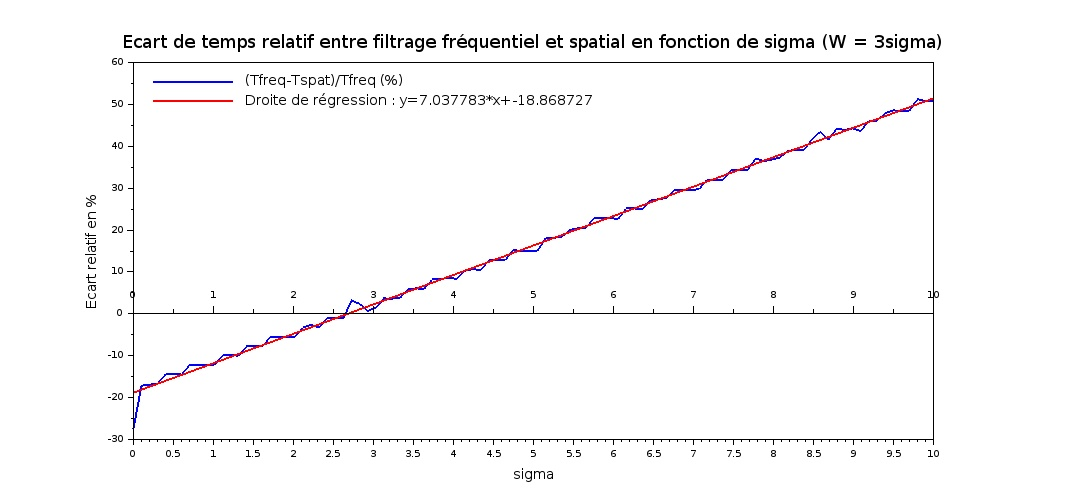
\includegraphics[width = 170mm]{./img/timeDiff.jpg}
\end{center}

On voit sur cette figure que pour de petites valeurs de $\sigma$, et donc une faible variance de gaussienne, le filtrage spatial est plus intéressant que le filtrage fréquentiel. En effet pour ces faibles tailles la taille du masque à utiliser est aussi petite, ce qui implique un nombre de calculs moindre (Le filtrage spatial est alors jusqu'à 20\% plus rapide).

Cette tendance s'inverse pour les valeurs de $\sigma$ importantes, c'est ici l'effet inverse qui se produit, le masque doit, pour ces valeurs, prendre une taille importante qui alourdit les calculs (jusqu'à 50\% plus lent que le filtrage fréquentiel pour $\sigma=10$).\\

\noindent
L'équivalence entre les deux méthodes se trouve à une taille proche de $\sigma = 2.5$. Ainsi :
\begin{itemize}
	\item Pour une taille $\sigma < 0.5$ c'est le filtrage \textit{spatial} qui est à privilégier
	\item A l'inverse, pour $\sigma \geq 0.5$ le filtrage \textit{fréquentiel} est celui qui minimise le temps de calcul
\end{itemize}


% Fin section 1 %
\section{Partie II : Détection de contours}

\subsection{Opérateurs différentiels du premier ordre}
L'idée ici est de définir le contour comme une forte variation de valeur locale. L'opérateur gradient permet justement d'évaluer les variations d'une application.
En considérant l'image comme une application on peut retrouver ses contours en cherchant les fortes valeurs de gradient.
Pour cela on approche le gradient de chaque pixel par une formule de différences finies et on fixe une valeur seuil à partir de laquelle on estime que le pixel appartient à un contour.
Sur la figure suivante on voit que la méthode est fonctionnelle.\\

\noindent
\begin{center}
\begin{minipage}[c]{0.20\linewidth}
	\begin{center}
		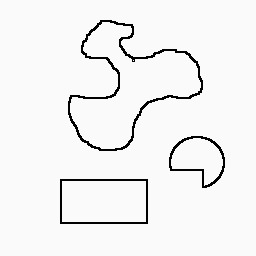
\includegraphics[width = 33mm]{./img/p2test_grad_mean_formes2.jpg}
		\textit{Détection de contours\\ forme 2}
	\end{center}
\end{minipage}
\end{center}

Ici, on a utilisé la seconde forme qui est une version moins contrastée de la première forme. En choisissant un seuil adapté on obtient bien les mêmes résultats pour les deux versions.
On peux donc estimer que la variation de contraste n'est pas un problème pour la détection de contours.\\
En revanche c'est désagréable d'avoir à ajuster le seuil on peux envisager de choisir une valeur qui s'adapterais au contraste de l'image.\\

bruits poivre et sel -> galère
\noindent
\begin{center}
\begin{minipage}[c]{0.20\linewidth}
	\begin{center}
		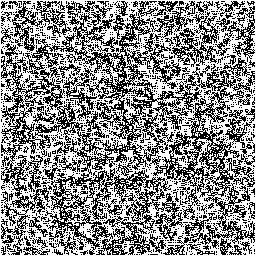
\includegraphics[width = 33mm]{./img/p2test_grad_mean_formes2pets5.jpg}
		\textit{origine}
	\end{center}
\end{minipage}
\end{center}

bruit spéculum -> les contour détécter fome de grosse tache.
\noindent
\begin{center}
\begin{minipage}[c]{0.20\linewidth}
	\begin{center}
		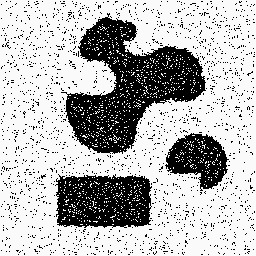
\includegraphics[width = 33mm]{./img/p2test_grad_mean_formes1sp.jpg}
		\textit{origine}
	\end{center}
\end{minipage}
\end{center}

bruit gaussien -> graduelement difficile : bon jusqu'a 30
\noindent
\begin{center}
\begin{minipage}[c]{0.20\linewidth}
	\begin{center}
		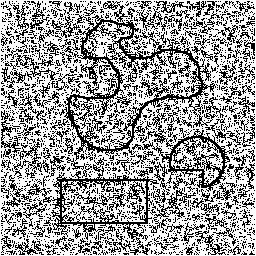
\includegraphics[width = 33mm]{./img/p2test_grad_mean_formes2bb10.jpg}
		\textit{Détection de contour \\bruit blanc 10}
	\end{center}
\end{minipage}
\end{center}
fonctionnement ...

\subsubsection{On peux fixer le seuil relativement à l'image}
A part certain cas extreme (voire ci-dessous) Choisire une valeur de seuil se rapportant à la moyenne
et un bon compromis. Cela évite à l'utilisateur de rechercher un seuil valable.
Bien sur on peux toujours améliorer le résultat en ajustant le seuil plus finement.\\
\noindent
\begin{center}
\begin{minipage}[c]{0.20\linewidth}
	\begin{center}
		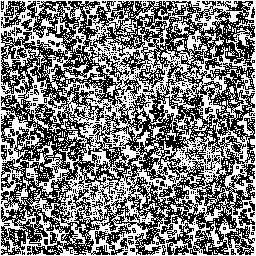
\includegraphics[width = 33mm]{./img/p2test_grad_mean_formes1pets5.jpg}
		\textit{Mean}
	\end{center}
\end{minipage}
\begin{minipage}[c]{0.20\linewidth}
	\begin{center}
		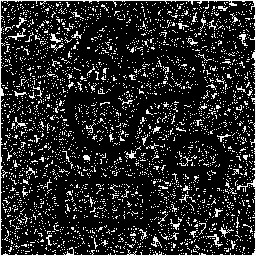
\includegraphics[width = 33mm]{./img/p2test_grad_const_formes1pets5.jpg}
		\textit{Seuil=20}
	\end{center}
\end{minipage}
\end{center}

\subsubsection{Commencer par filtrer l'image}
\noindent
\begin{center}
\begin{minipage}[c]{0.20\linewidth}
	\begin{center}
		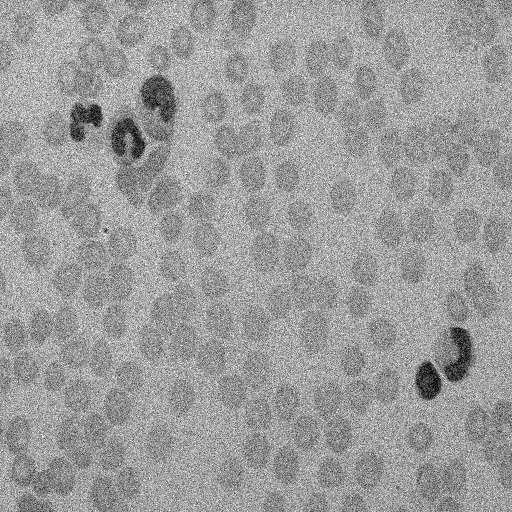
\includegraphics[width = 33mm]{./img/globulesbb26.jpg}
		\textit{Image original : bruit gaussien 26}
	\end{center}
\end{minipage}
\begin{minipage}[c]{0.20\linewidth}
	\begin{center}
		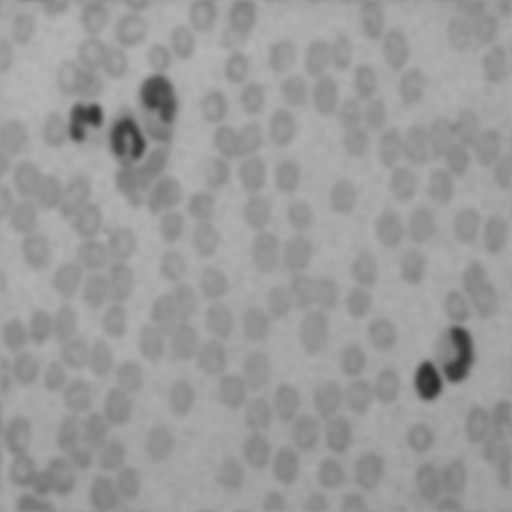
\includegraphics[width = 33mm]{./img/globulesbb26_filtrer3.jpg}
		\textit{Image filtrée \\ $\sigma=3$}
	\end{center}
\end{minipage}
\end{center}


\noindent
\begin{center}
\begin{minipage}[c]{0.20\linewidth}
	\begin{center}
		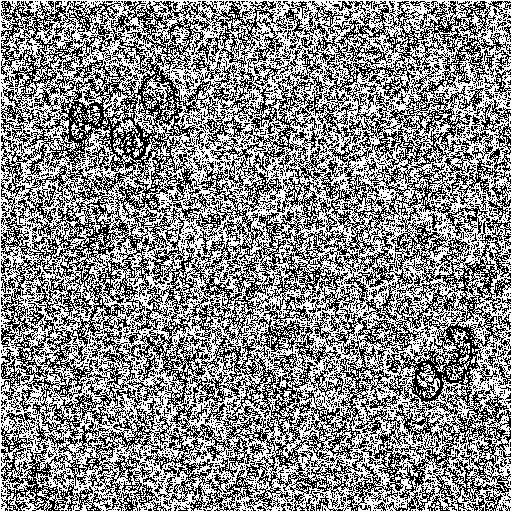
\includegraphics[width = 33mm]{./img/globulesbb26_mean.jpg}
		\textit{Detection de contour sur l'image original}
	\end{center}
\end{minipage}
\begin{minipage}[c]{0.20\linewidth}
	\begin{center}
		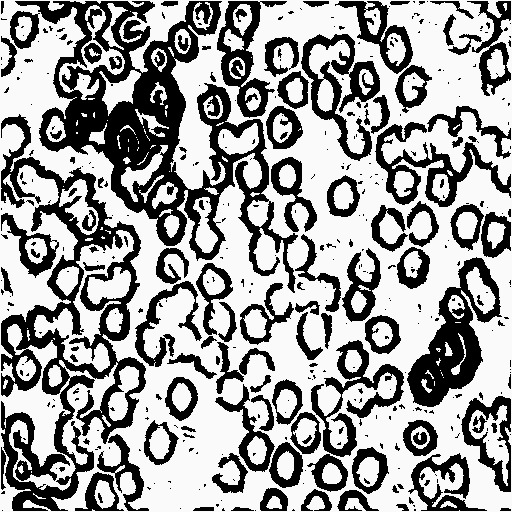
\includegraphics[width = 33mm]{./img/globulesbb26_filtrer3_mean.jpg}
		\textit{Detection de contour sur l'image filtrée}
	\end{center}
\end{minipage}
\end{center}



\subsubsection{Second ordre approché}
Le probleme principal de cette première détection de contour, Que le filtrage préléminaire accentue, est la largeur des contours.
En effet, Détecter un contour n'est pas uniquement trouver sont existance. c'est aussi en connaitre la localisation. Or lorsque le contour et représenté par une
lagre bande de pixel, il est difficile de conaitre précisément où le positionner.\\

\noindent
\begin{minipage}[c]{0.20\linewidth}
	\begin{center}
		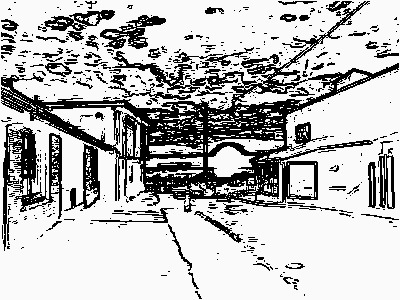
\includegraphics[width = 33mm]{./img/p2test_grad_mean_soleil.jpg}
		\textit{coucher de Soleil}
	\end{center}
\end{minipage}
\begin{minipage}[c]{0.20\linewidth}
	\begin{center}
		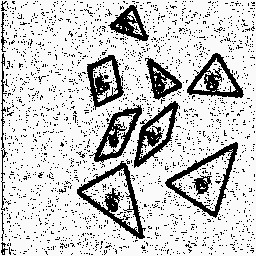
\includegraphics[width = 33mm]{./img/p2test_grad_mean_tangram.jpg}
		\textit{tangram}
	\end{center}
\end{minipage}
\begin{minipage}[c]{0.20\linewidth}
	\begin{center}
		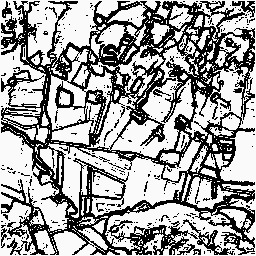
\includegraphics[width = 33mm]{./img/p2test_grad_mean_aquitain.jpg}
		\textit{aquitain}
	\end{center}
\end{minipage}
\begin{minipage}[c]{0.20\linewidth}
	\begin{center}
		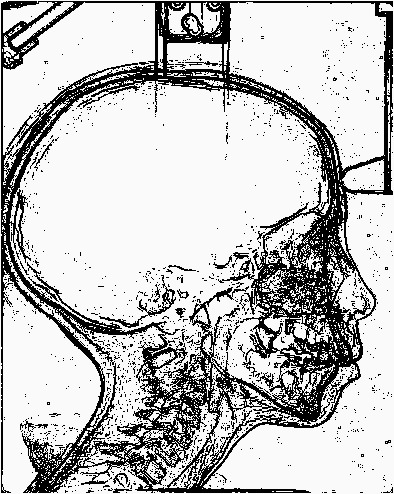
\includegraphics[width = 33mm]{./img/p2test_grad_mean_radio1.jpg}
		\textit{radio}
	\end{center}
\end{minipage}
\begin{minipage}[c]{0.20\linewidth}
	\begin{center}
		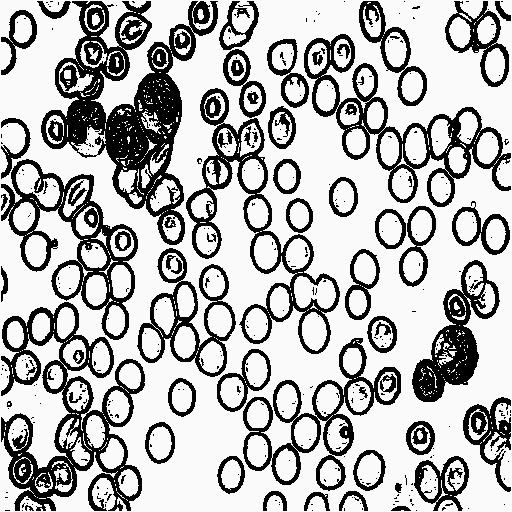
\includegraphics[width = 33mm]{./img/p2test_grad_mean_globules.jpg}
		\textit{globules}
	\end{center}
\end{minipage}

\noindent
\begin{minipage}[c]{0.20\linewidth}
	\begin{center}
		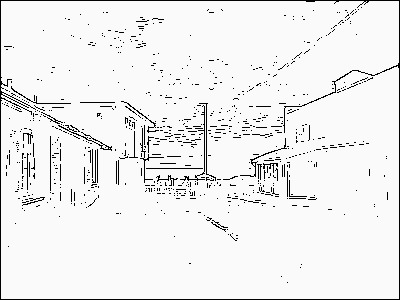
\includegraphics[width = 33mm]{./img/p2test_grad_fin_soleil.jpg}
		\textit{coucher de soleil}
	\end{center}
\end{minipage}
\begin{minipage}[c]{0.20\linewidth}
	\begin{center}
		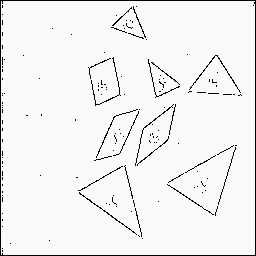
\includegraphics[width = 33mm]{./img/p2test_grad_fin_tangram.jpg}
		\textit{tangram}
	\end{center}
\end{minipage}
\begin{minipage}[c]{0.20\linewidth}
	\begin{center}
		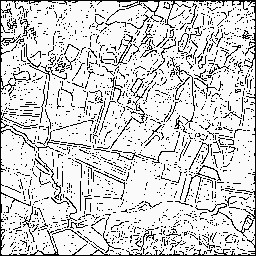
\includegraphics[width = 33mm]{./img/p2test_grad_fin_aqitain.jpg}
		\textit{aquitain}
	\end{center}
\end{minipage}
\begin{minipage}[c]{0.20\linewidth}
	\begin{center}
		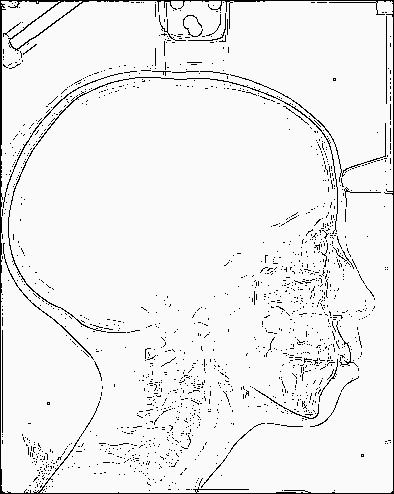
\includegraphics[width = 33mm]{./img/p2test_grad_fin_radio.jpg}
		\textit{radio}
	\end{center}
\end{minipage}
\begin{minipage}[c]{0.20\linewidth}
	\begin{center}
		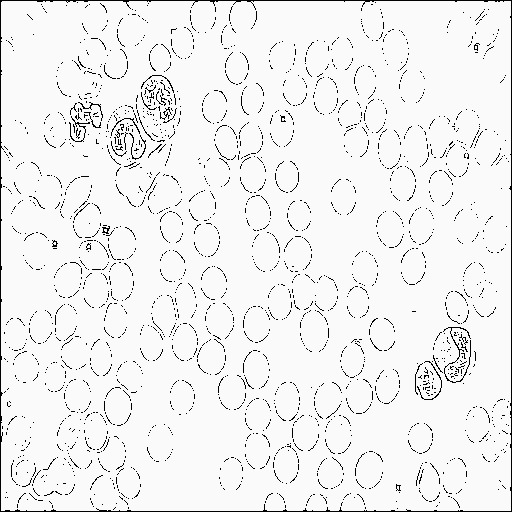
\includegraphics[width = 33mm]{./img/p2test_grad_fin_globules_t10.jpg}
		\textit{globules}
	\end{center}
\end{minipage}


cela introduit une nouvelle forme de seuil.\\
\noindent
\begin{center}
\begin{minipage}[c]{0.20\linewidth}
	\begin{center}
		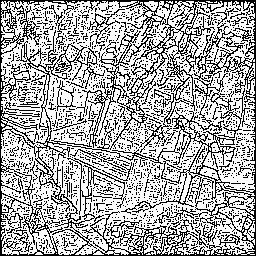
\includegraphics[width = 33mm]{./img/p2test_grad_fin_aqitain_t1.jpg}
		\textit{t=1}
	\end{center}
\end{minipage}
\begin{minipage}[c]{0.20\linewidth}
	\begin{center}
		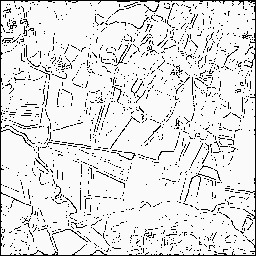
\includegraphics[width = 33mm]{./img/p2test_grad_fin_aqitain_t5.jpg}
		\textit{t=5}
	\end{center}
\end{minipage}
\begin{minipage}[c]{0.20\linewidth}
	\begin{center}
		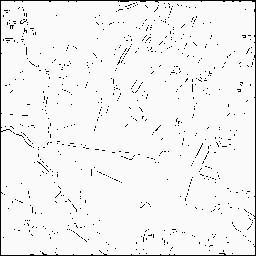
\includegraphics[width = 33mm]{./img/p2test_grad_fin_aqitain_t10.jpg}
		\textit{t=10}
	\end{center}
\end{minipage}
\end{center}

Cependant le moindre bruit rend cette nouvelle méthode inefficace.\\
\noindent
\begin{minipage}[c]{0.10\linewidth}
	\begin{center}
		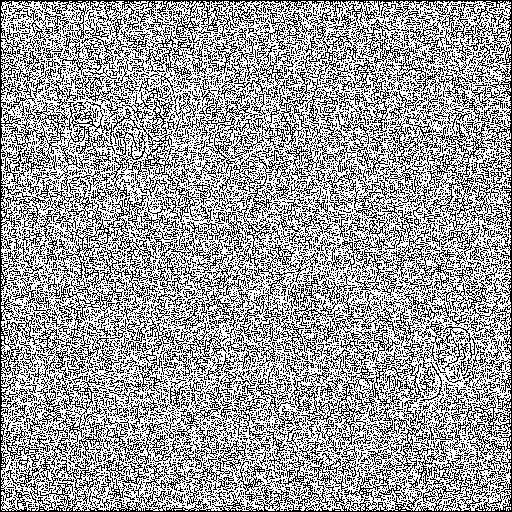
\includegraphics[width = 25mm]{./img/p2test_grad_fin_globules10_t3.jpg}
		\textit{t=3}
	\end{center}
\end{minipage}
\begin{minipage}[c]{0.10\linewidth}
	\begin{center}
		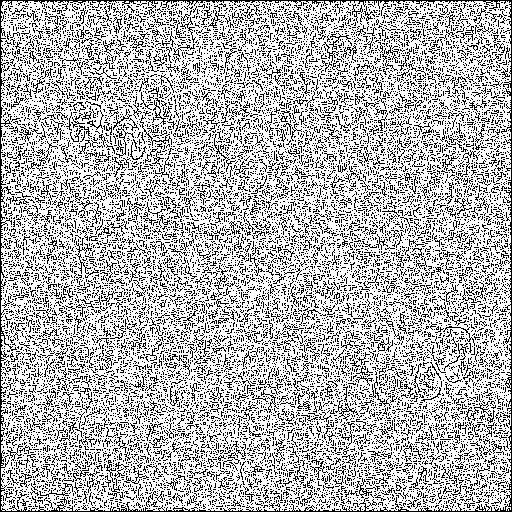
\includegraphics[width = 25mm]{./img/p2test_grad_fin_globules10_t15.jpg}
		\textit{t=15}
	\end{center}
\end{minipage}
\begin{minipage}[c]{0.10\linewidth}
	\begin{center}
		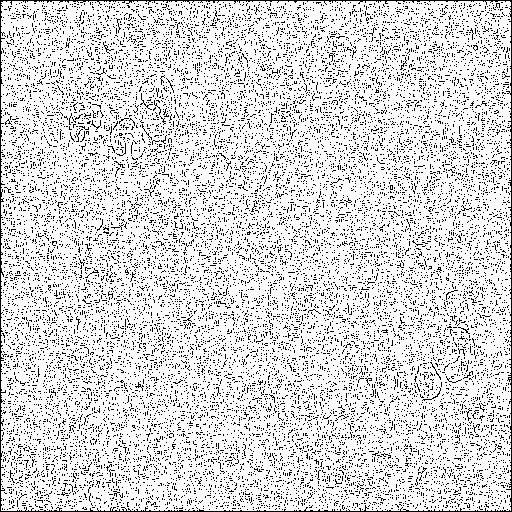
\includegraphics[width = 25mm]{./img/p2test_grad_fin_globules10_t25.jpg}
		\textit{t=25}
	\end{center}
\end{minipage}
\begin{minipage}[c]{0.10\linewidth}
	\begin{center}
		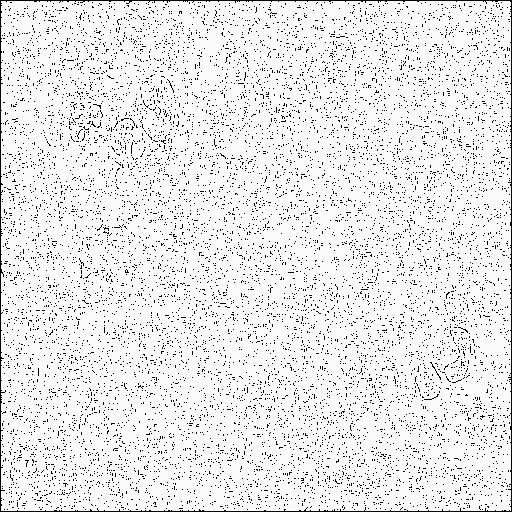
\includegraphics[width = 25mm]{./img/p2test_grad_fin_globules10_t35.jpg}
		\textit{t=35}
	\end{center}
\end{minipage}
\begin{minipage}[c]{0.10\linewidth}
	\begin{center}
		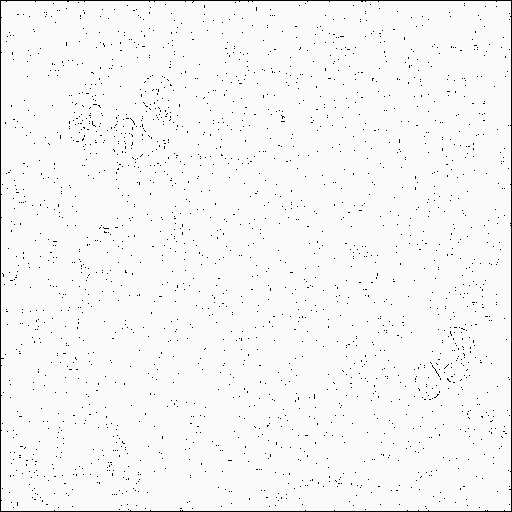
\includegraphics[width = 25mm]{./img/p2test_grad_fin_globules10_t55.jpg}
		\textit{t=55}
	\end{center}
\end{minipage}
\hspace{2cm}
$\longrightarrow$
\hspace{1cm}
\begin{minipage}[c]{0.10\linewidth}
	\begin{center}
		\includegraphics[width = 33mm]{./img/globulesbb10_filtre2_fin1.jpg}
		\textit{filtre $\sigma=2$ et t=1}
	\end{center}
\end{minipage}



\subsection{Opérateurs différentiels du deuxième ordre}
Pour l'implémentation de la détection de contours par opérateurs du second ordre nous avons choisi d'implémenter le filtre passe-bande LoG par FFT. Nous n'avons pas utilisé un filtre idéalisé mais un filtre sous la forme $\mathcal{F}(\Delta G_{\sigma})$, où le paramètre $\sigma$ peut être choisi.\\


L'image du laplacien obtenue par cette méthode doit ensuite être traitée pour détecter les passages par zéro. Pour cela nous avons remarqué plusieurs choses lors de notre implémentation :
\begin{itemize}
	\item Il n'est pas possible de chercher les zéros de l'image, en effet les valeurs étant discrétisées et les calculs n'étant pas exacts il est très peu probable de trouver le passage par zéro de cette manière. Il est donc nécessaire de détecter un \textit{changement de signe} du laplacien.
	\item En regardant la \textit{Figure 5} du sujet on voit que le laplacien est très proche de zéro en l'absence de contours (pas ou peu de variations d'intensité, et donc très faible valeur au second ordre) et ces changements de signes sont donc susceptibles d'arriver dans ces zones. Il a donc été nécessaire de ne détecter que les changements de signe entre des valeurs espacées d'une certaine amplitude. Nous avons fixé empiriquement ce seuil à 1.\\
\end{itemize}

On remarque tout d'abord que sur des images simples et sans bruit telles que les images \textit{formes1/2.pgm} le filtre offre une très bonne détection (résultat identique sur les deux contrastes) avec une valeur de $\sigma$ adaptée :\\

\noindent
\begin{center}
	\begin{minipage}[c]{0.24\linewidth}
		\begin{center}
			\includegraphics[width = 40mm]{./img/1.jpg}
			\textit{origine}
		\end{center}
	\end{minipage}
	\begin{minipage}[c]{0.24\linewidth}
		\begin{center}
			\includegraphics[width = 40mm]{./img/ctrformes1-0_5.jpg}
			\textit{$\sigma = 0.5$}\
		\end{center}
	\end{minipage}
	\begin{minipage}[c]{0.24\linewidth}
		\begin{center}
			\includegraphics[width = 40mm]{./img/ctrformes1-1.jpg}
			\textit{$\sigma = 1$}
		\end{center}
	\end{minipage}
	\begin{minipage}[c]{0.24\linewidth}
		\begin{center}
			\includegraphics[width = 40mm]{./img/ctrformes1-2_5.jpg}
			\textit{$\sigma = 2_.5$}
		\end{center}
	\end{minipage}\\
\end{center}

Ainsi :
\begin{itemize}
	\item Pour une valeur de $\sigma$ trop faible les contours détectées sont trop gros et des doubles détections espacées apparaissent.
	\item Pour une valeur trop élevée au contraire des bouts de contours disparaissent et des défauts apparaissent (visibles au niveau des angles droits du rectangle notamment) jusqu'à qu'aucun contour ne soit plus détecté.\\
\end{itemize}


L'addition de bruit, comme prédit avec la \textit{Figure 4} du sujet rend la méthode très instable, du fait de l'utilisation d'opérateurs du second ordre. L'utilisation du filtre gaussien en amont de la détection, comme présenté pour la détection par gradient ne permet pas ici de grande amélioration.

En effet même si le bruit est atténué, l'étalement des contours oblige à choisir un $\sigma$ plus grand pour le calcul du laplacien, et l'image résultante est pratiquement identique à celle obtenue sans filtrage. Nous allons illustrer cela sur l'image \textit{globules}.\\\\

\textbf{Image sans bruit :}

\begin{center}
	\begin{minipage}[c]{0.49\linewidth}
		\begin{center}
			\includegraphics[width = 80mm]{./img/globules.jpg}\\
			\textit{origine}\\
		\end{center}
	\end{minipage}
	\begin{minipage}[c]{0.49\linewidth}
		\begin{center}
			\includegraphics[width = 80mm]{./img/ctrglobules-1_2.jpg}\\
			\textit{$\sigma = 1.2$}\\
		\end{center}
	\end{minipage}
\end{center}

Sur cette image sans bruit il est possible d'arriver à une très bonne détection des contours.\\

\textbf{Image bruitée (\textit{globulesbb26}) :}

\begin{center}
	\begin{minipage}[c]{0.49\linewidth}
		\begin{center}
			\includegraphics[width = 80mm]{./img/globulesbb26.jpg}\\
			\textit{origine}\\
		\end{center}
	\end{minipage}
	\begin{minipage}[c]{0.49\linewidth}
		\begin{center}
			\includegraphics[width = 80mm]{./img/ctrglobulesbb26-2_2.jpg}\\
			\textit{détection laplacien : $\sigma = 2.2$}\\
		\end{center}
	\end{minipage}
\end{center}

\begin{center}
	\begin{minipage}[c]{0.49\linewidth}
		\begin{center}
			\includegraphics[width = 80mm]{./img/globulesbb26fg-2.jpg}\\
			\textit{filtre gaussien : $\sigma = 2$}\\
			\textit{}
		\end{center}
	\end{minipage}
	\begin{minipage}[c]{0.49\linewidth}
		\begin{center}
			\includegraphics[width = 80mm]{./img/globulesbb26fg-2-ctr-1.jpg}\\
			\textit{détection laplacien ($\sigma = 1$) avec filtrage précédent ($\sigma = 2$): }\\
		\end{center}
	\end{minipage}
\end{center}

Exemples obtenus sur les images de test :
\begin{center}
	\begin{minipage}[c]{0.30\linewidth}
		\begin{center}
			\includegraphics[width = 50mm]{./img/aquitain.jpg}
			\textit{origine}\\
		\end{center}
	\end{minipage}
	\begin{minipage}[c]{0.30\linewidth}
		\begin{center}
			\includegraphics[width = 50mm]{./img/couchersoleil.jpg}
			\textit{origine}\\
		\end{center}
	\end{minipage}
	\begin{minipage}[c]{0.30\linewidth}
		\begin{center}
			\includegraphics[width = 50mm]{./img/radio.jpg}
			\textit{origine}\\
		\end{center}
	\end{minipage}
\end{center}

\begin{center}
	\begin{minipage}[c]{0.30\linewidth}
		\begin{center}
s			\includegraphics[width = 50mm]{./img/ctraquitain-1.jpg}
			\textit{$\sigma = 1$}\\
		\end{center}
	\end{minipage}
	\begin{minipage}[c]{0.30\linewidth}
		\begin{center}
			\includegraphics[width = 50mm]{./img/ctrcouchersoleil-1_5.jpg}
			\textit{$\sigma = 1.5$}\\
		\end{center}
	\end{minipage}
	\begin{minipage}[c]{0.30\linewidth}
		\begin{center}
			\includegraphics[width = 50mm]{./img/ctrradio-1_5.jpg}
			\textit{$\sigma = 1.5$}\\
		\end{center}
	\end{minipage}
\end{center}


\subsection{Comparaison}
Comme nous l'avons vu dans les parties précédentes on peut extraire des caractéristiques propres aux deux méthodes :
\begin{itemize}
	\item La détection par laplacien est bien plus sensible au bruit que la détection par gradient
	\item Les images bruitées nécessitent invariablement un traitement de dé-bruitage avec un filtre de détection de contours sous peine de fausse cette détection.
	\item Du fait de son fonctionnement par détection des passages par zéro avec un certain seuil, le laplacien permet d'obtenir des contours souvent plus fins que ceux obtenus par une méthode du gradient
	\item Cela le rend cependant bien moins réceptif au pré-filtrage par filtre gaussien qui permet une réduction du bruit au prix d'un élargissement des contours. Cela conduit à un grossissement des contours pour la détection par gradient mais à une forte difficulté de détection par laplacien (étalement et donc seuillage difficile pour la détection du passage par zéro)\\
\end{itemize}

Nous pouvons voir l'épaisseur des contours détectés sur l'exemple de l'image \textit{couchersoleil.pgm} :

\begin{center}
	\begin{minipage}[c]{0.49\linewidth}
		\begin{center}
			\includegraphics[width = 80mm]{./img/p2test_grad_mean_soleil.jpg}\\
			\textit{détection par gradient}\\
		\end{center}
	\end{minipage}
	\begin{minipage}[c]{0.49\linewidth}
		\begin{center}
			\includegraphics[width = 80mm]{./img/ctrcouchersoleil-1_5.jpg}\\
			\textit{détection par laplacien}\\
		\end{center}
	\end{minipage}
\end{center}

\vspace{2em}
Enfin la détection en présence de bruit (avec filtrage préalable) est mieux gérée par l'opérateur de gradient, nous pouvons comparer cela sur l'image : \textit{globulesbb26.pgm} :
\begin{center}
	\begin{minipage}[c]{0.49\linewidth}
		\begin{center}
			\includegraphics[width = 80mm]{./img/globulesbb26_filtrer3.jpg}\\
			\textit{détection par gradient}\\
		\end{center}
	\end{minipage}
	\begin{minipage}[c]{0.49\linewidth}
		\begin{center}
			\includegraphics[width = 80mm]{./img/globulesbb26fg-2-ctr-1.jpg}\\
			\textit{détection par laplacien}\\
		\end{center}
	\end{minipage}
\end{center}


% Fin section 2 %
\end{document}

% Fin du document LaTeX
